\chapter{Reporting in the Poisson process context.}

\section{Modeling observed reporting data.}

The reporting delays, $t_d$, are observed.  These can be modelled
directly as, for example, having a weibull distribution.  To estimate
such a model we would:

\begin{enumerate}
\item load all data with the columns: \begin{itemize}
	\item $t_r$, the date of the report delivery.
	\item $t_s$, the date of illness.
	\item $t_d=t_r - t_s$, the reporting delay.
	\item $j$, the province.
	\end{itemize}
\end{enumerate}

Weibull model in Stan..., etc...

This lets us estimate parameter for a posterior density
$p(t_d|\theta_d)$.  

\section{The reporting problem in the Poisson process model.} 

The question we want to answer to integrate the reporting model with a
disease dynamics model is: 

Q1: What proportion of cases which occur between time point $t_a$ and
$t_b$ are reported by $t^*$.

Knowing this fraction, $f(t^*, t_a, t_b)$, would let us convert $y$, the
case count observed between time points $t_a$ and $t_b$, into $y^*$, the true (or reporting-adjusted) case
count.  

\begin{equation}
y = y^* \times f(t^*, t_a, t_b)
\end{equation}

It is likely that this is some kind of CDF for $t^*$, but it's
form is unclear. To get there we start by asserting that we will specify
two densities: one for the reporting/delay process and one for the
disease process:

\begin{align}
p_d(t_d|\theta_d) &= \ldots \\
p_s(t_s|\theta_s) &= \ldots
\end{align}

The disease process is a primary focus of this work and the poisson
process model can be used to estimate an intensity function as
described.  The density function for the dates of illness ($t_s$) is
(the same?) a transformation of the intensity function.

The reporting delays are directly observed and standard time-to-event
modeling techniques can be applied to estimate the parameters of the
density of $t_d$.  Due to the deterministic relationship between $t_r$
and $t_s$, we can specify a distribution for $t_r$ conditional on $t_s$.

\begin{equation}
p_r(t_r|\theta_d, t_s) = p_d(t_r - t_s| \theta_d) 
\end{equation}

To remove the conditionality on $t_s$, we can construct the joint
distribution for $p_{r,s}$ and integrate over the
possible values.  In the poisson process, counts are reported in batches
which begin at $a$ and end at $b$ restricting $t_a < t \le  t_b$,
and these are the relevant bounds for integration:

\begin{align}
p_{r,s}(t_r, t_s| \theta_d, \theta_s) = p_s(t_s|\theta_s) p_r(t_r|\theta_d, t_s) \\
p_r(t_r|\theta_d, \theta_s, a<t\le b) = \int_a^b p_s(t_s|\theta_s) p_r(t_r|\theta_d, t_s)
\end{align}

The resulting density is depends only on the parameters of the reporting
model ($\theta_d$), the disease model ($\theta_s$), and the boundaries
of the batch ($t \in [a,b)$).  This density defines the distribution of
reporting times for a batch of cases.  For cases to be available for a
model, they must be reported prior to, $t^*$,  the time of the analysis.  
The proportion of available cases can be stated in terms of the CDF: 

\begin{equation}
Pr[t_r < t^*| \theta_d, \theta_s, a<t\le b] = \int_a^{t^*} p_r(t_r|\theta_d, \theta_s, a<t<=b) dt_r
\end{equation}

Which lets us relate $y$ and $y^*$.

\begin{equation}
y = y^* \times Pr[t_r < t^*| \theta_d, \theta_s, a<t\le b]
\end{equation}

\section{Reasonable approximations to the rescue}

One difficulty with this approach is that we do not have an analytical
expression for $p_s$ (or its integral), which means we do not
have an analytical expression for $p_r$ (or its integral).  We begin
with an approximation of the disease process.  

First assume that $a$ and $b$ generate an interval short enough such
that $p_s$ is apprximately flat over this interval.  This requires that
counts for each batch are collected over a short period of time.  Then 

\begin{align}
t_s \sim U(a,b) \\
p(t_s|\theta_s, a^*, b^*) \sim \frac{1}{b^* - a^*}
\end{align}

If we also assume a Weibull distribution for the reporting
interval/delay, we can get an approximate density for $t_r$.

\begin{align}
p(t_r| \theta_d, t_s) &= k\lambda(t_d\lambda)^{k-1} e^{-(x\lambda)^k} \\
p(t_r| \theta_d, \theta_s, a < t_s \le  b) 
		&= \int_a^b p_s(t_s|\theta_s) p_r(t_r|\theta_d, t_s) dt_s\\
		&= \int_a^b \frac{1}{b^*-a^*} k\lambda(t_d\lambda)^{k-1} e^{-(t_d\lambda)^k} dt_s\\
		&= \frac{1}{b^*-a^*} \int_a^b \text{PDF}_{t_d}(t_r - t_s) dt_s\\
		&= \frac{1}{b^*-a^*} \big[ \text{CDF}_{t_d}(t_r-a|k,\lambda) - \text{CDF}_{t_d}(t_r-b|k,\lambda) \big]
\end{align}

Since the delays are in reverse-time, we flip integral bounds to get a positive
PDF function for $t_r$. Any model for $t_d$ which has an PDF with a
matching known CDF in closed form can be put through the same process.
The result is a scaled version of the original PDF with expanded
variance.



\begin{knitrout}
\definecolor{shadecolor}{rgb}{0.969, 0.969, 0.969}\color{fgcolor}\begin{kframe}
\begin{alltt}
\hlstd{pl} \hlkwb{<-} \hlkwd{readRDS}\hlstd{(}\hlkwc{file}\hlstd{=}\hlkwd{file.path}\hlstd{(figure_dir,} \hlstr{'reporting-approximation.rds'}\hlstd{))}
\hlkwd{print}\hlstd{(pl)}
\end{alltt}
\end{kframe}\begin{figure}[]

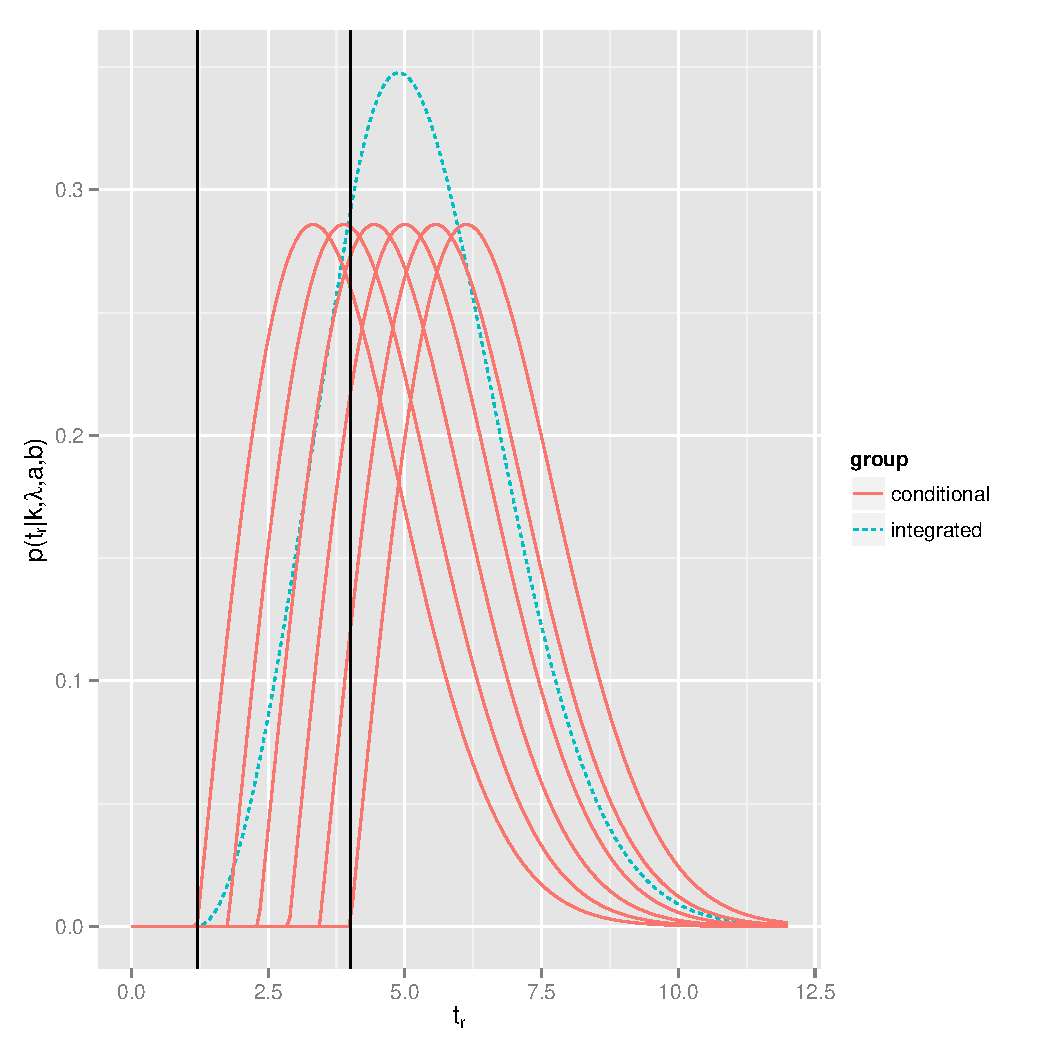
\includegraphics[width=\maxwidth]{figure/reporting-approximation-plot} \caption[Density for reporting dates, ($t_r$, shown with a dashed blue line), conditional on Weibull reporting delay distribution (shown in solid red lines) and bounds on the dates of illness ($a < t_s \le  b$, vertical lines)]{Density for reporting dates, ($t_r$, shown with a dashed blue line), conditional on Weibull reporting delay distribution (shown in solid red lines) and bounds on the dates of illness ($a < t_s \le  b$, vertical lines).\label{fig:reporting-approximation-plot}}
\end{figure}


\end{knitrout}

This gives us a closed-form solution for $t_r$, the density of reporting
times.  The final step is integrating this to get an expression for
$Pr[t_r < t^*| \theta_d, \theta_s, a<t\le b]$...

\begin{align}
Pr[&t_r < t^*| \theta_d, \theta_s, a<t\le b] =  \\
	&= \frac{1}{b^*-a^*} \Bigg[ 
		\int_a^{t^*} \text{CDF}_{t_d}(t_r-a|k,\lambda) - 
		\int_b^{t^*} \text{CDF}_{t_d}(t_r-b|k,\lambda) 
		\Bigg] \\
	&= \frac{1}{b^*-a^*} \Bigg[ 
		\int_a^{t^*} 1-e^{-([t_r-a]\lambda)^k} dt_r - \int_b^{t^*} 1-e^{-([t_r-b]\lambda)^k} dt_r 
	\Bigg] \\
	&= \frac{1}{b^*-a^*} \Bigg[ 
		\int_a^{t^*} 1 dt_r - \int_a^{t^*} e^{-([t_r-a]\lambda)^k} dt_r -
		\int_b^{t^*} 1 dt_r + \int_b^{t^*} e^{-([t_r-b]\lambda)^k} dt_r 
	\Bigg] \\
	&= \frac{1}{b^*-a^*} \Bigg[
		b - a +
		\int_a^{t^*} e^{-([t_r-a]\lambda)^k} dt_r +
		\int_b^{t^*} e^{-([t_r-b]\lambda)^k} dt_r 
	\Bigg] \\
\end{align}

The integrals can be rewritten in terms of incomplete upper gamma
functions.

\begin{align}
		\int_a^{t^*} & e^{-([t_r-a]\lambda)^k} dt_r = \\
			& \frac{(a-t^*)\Gamma(\frac{1}{k},[(t^*-a)\lambda]^k)}{(t^*-a)\lambda} -
			  \frac{(a-a  )\Gamma(\frac{1}{k},[(a  -a)\lambda]^k)}{ a  -a \lambda} = \\
			& -\frac{\Gamma(\frac{1}{k},[(t^*-a)\lambda]^k)}{\lambda} -
			  \frac{\Gamma(\frac{1}{k})}{\lambda} = \\
			& -\frac{1}{\lambda} \Bigg[
				\Gamma\bigg(\frac{1}{k},[(t^*-a)\lambda]^k\bigg) -
				\Gamma\bigg(\frac{1}{k}\bigg)
				\Bigg] = \\
			& \frac{1}{\lambda} \gamma\bigg(\frac{1}{k},\big[\lambda(t^*-a)\big]^k\bigg)
\end{align}

Which leaves the final expression as:

\begin{align}
Pr[&t_r < t^*| \theta_d, \theta_s, a<t\le b] =  \\
	&= \frac{1}{b^*-a^*} \Bigg[
		b - a +
		\int_a^{t^*} e^{-([t_r-a]\lambda)^k} dt_r +
		\int_b^{t^*} e^{-([t_r-b]\lambda)^k} dt_r 
	\Bigg] = \\
	&= \frac{1}{b^*-a^*} \Bigg[
		b - a + \frac{1}{\lambda} \bigg(
			\gamma\big(k^{-1},\big[\lambda(t^*-a)\big]^k\big) + 
			\gamma\big(k^{-1},\big[\lambda(t^*-b)\big]^k\big)
		\bigg)
	\Bigg]
\end{align}

This can be implemented in Stan for each instance of the incomplete
lower gamma function ($\gamma(a,x)$) by using the product of the normalized lower
incomplete gamma function (\verb#gamma_p#) and the gamma function
(\verb#tgamma#).  The equivalent is available in R and a more efficient 
method may be available (after all the outcome of this difference in
incomplete lower gamma functions is an integral over the scaled duration
of the interval during which the batch was reported).



